\documentclass[10pt,twocolumn]{article}

% formatting
\paperwidth=8.55in
\paperheight=11in
\setlength{\columnsep}{0.25in}
\usepackage{leading}
\usepackage[margin=0.7in]{geometry}

\usepackage{times}
\usepackage{listings, textcomp}
\usepackage[T1]{fontenc}

\usepackage{amsmath}
\usepackage{booktabs}
\usepackage{graphicx}
\usepackage{enumitem}
\usepackage[hidelinks]{hyperref}
\hypersetup{breaklinks=true}
\Urlmuskip=0mu plus 2mu
\usepackage{subcaption}
\usepackage{xcolor}

\newcommand{\remark}[1]{{\color{red}[#1]}}

\begin{document}

\leading{11pt}

\title{\bf Contextual Code Completion Using Machine Learning}
\author{Subhasis Das, Chinmayee Shah\\
        \{subhasis,~chshah\}@stanford.edu\\
        Mentor: Junjie Qin}

\date{}
\maketitle
\thispagestyle{empty}

\section{Introduction}
\label{sec:intro}

\noindent
Code IDEs such as Eclipse and Microsoft Visual Studio make the task of writing
code in new languages easier by auto-completing key words and phrases.
For example, when writing code in C++, an IDE may automatically close an
opening parenthesis, and suggest else immediately following an if block.
Such code completion has several problems:
\begin{enumerate}[topsep=0pt,itemsep=-1ex,partopsep=1ex,parsep=1ex]
  \item Grammar based code completion requires writing down an exhaustive set
    of rules. This is tedious and repetitive when done for every new language.
  \item Predictions do not consider the category of code. For instance, driver
    codes and math libraries may exhibit different patterns.
  \item Predictions do not consider context such as header file, class
    definition, function definition, tabs and spaces, opening and closing
    braces on the same line.
  \item Recommendations are often ordered lexicographically, which means some
    of the top recommendations may not be useful.
\end{enumerate}

\noindent
This report explores a learning based approach to code completion. Instead of
writing grammar based rules, we use machine learning to learn structure and
patterns in code. We can then not only automate code predictors for different
languages, but also specialize them for different kinds of projects such as
drivers and libraries. We can also consider the enclosing context and rank
predictions.
%Section~\ref{sec:model} describes our model for the problem of code completion.
%It also gives a brief overview of a word vector based approach to modeling
%tokens in code, and techniques we use to work with a limited volcabulary of
%words.
%Section~\ref{sec:memoryless} presents memoryless techniques for predicting
%based on only a small window of preceeding tokens. While these techniques use
%less contextual information, we can still train them for different languages
%and projects.
%Section~\ref{sec:window} presents results about the influence of different
%tokens on the output.
%Section~\ref{sec:conclusions} presents conclusions about the techniques that we
%have explored so far, and proposes stateful techniques for using more immediate
%context such as file based context to improve predictions.

%\vspace{-5pt}
\section{Modeling Tokens}
\label{sec:model}

\noindent
One of our objectives of learning based code prediction is to do away with the
tedious process of building grammar based rules for different languages.
We treat codes in the training set in a language agnostic way. The first step
is to build a dictionary of tokens or words that can occur in the code, that we
can take as input to predict the next token. We build this dictionary by
reading all code, and treating each consecutive set of alphanumeric characters
and (\_), or each consecutive set of special characters other than alphanumeric,
(\_), space and newline as one token.  Thus, for example, the code {\tt for
(my\_var = 0; my\_var < foo; my\_var++) \{} will be tokenized into eleven
tokens: {\tt for}, {\tt my\_var}, {\tt =}, {\tt 0}, {\tt ;}, {\tt my\_var}, {\tt
<}, {\tt foo}, {\tt;}, {\tt my\_var}, {\tt++) \{}.  Given a sequence of tokens, we
then want to predict the next token. Note that these tokens do not correspond
exactly to language level tokens, e.g., {\tt++) \{} is a single token despite
containing three different language level tokens {\tt++}, {\tt)}, and
{\tt\{}.

The dictionary of tokens constructed as above is not complete, since new code
may contain new tokens that are not present in the training data. Moreover,
many of the tokens in the training data may be specific to a few files and may
never occur again. To address these issues, we divide the tokens into two
categories:

a) {\it Key tokens}: A subset of $K$ most frequent tokens are categorized as
{\it key tokens}. Not surprisingly, many of
these frequent tokens are keywords for the language the project is written in,
or words that tend to occur often in that
particular project.
For example, some of the frequent tokens in Linux kernel are:
\texttt{struct}, \texttt{;}, and \texttt{dev}, out of which the first and second
are keywords in C, and the third is a token frequently used to denote device
objects in Linux. Note that while several language keywords do end up being part
of the set of key tokens, we {\it do not} manually curate the list of key tokens
to ensure that they contain only language specific keywords.

b) {\it Positional Tokens}: While key tokens occurrences constitute a major
fraction of all token occurrences ($\approx$ 60\% with 2000 key tokens),
the remainder of tokens are rarely
seen (such as names of variables, macros etc.). However, we would like our
learning algorithm to autocomplete new variable names, once they occur in a
file. For
example, given many examples of the form {\tt for (int TOKEN = 0; TOKEN < n;
TOKEN++)} (all with different values of {\tt TOKEN}), our algorithm should be
able to autocomplete {\tt for (int myIterName = 0;} with {\tt myIterName}. This
capability can not be achieved by merely trying to autocomplete between a set of
pre-defined key tokens. Hence, we also define {\it positional tokens} as follows.

Given a sequence of tokens --- an incomplete piece of code, we replace each
token which is not a key token by a string of the form {\tt
POS\_TOK\_ii}, where {\tt ii} is the {\it position} of that token
within that sequence. A non-keyword token which is repeated multiple times in a
sequence is assigned the index corresponding to its first appearance. For
example, given the sequence of tokens {\tt[for, int, myVarName, =, 0, ;,
myVarName, <, n, ;, myVarName, ++]}, where {\tt myVarName} is not a key token,
we construct the new sequence {\tt[for, int, POS\_TOK\_2, =, 0, ;, POS\_TOK\_2,
<, n, ;, POS\_TOK\_2, ++]}. In case the token to be predicted is not a key token
but has appeared in the window, it is also replaced by the corresponding
positional token string. If the target has not appeared before in the window, it
is assumed to be a special token {\tt UNKNOWN}. However, as we describe in
Section~\ref{sec:methods}, we ignore such windows since in many such
cases the token is actually a hereto unseen token.

Such an encoding is advantageous since now the set of prediction targets to
choose from is simply the union of the key tokens and the positional token
strings (of the form {\tt POS\_TOKEN\_ii}). In case of a fixed window size of
$W$ and a fixed number of key tokens $K$, it can be seen that the total number
of prediction targets is $K+W+1$ ($K$ key tokens, $W$ positional tokens, and 1
unknown token), i.e., a {\it constant}. This immediately opens up the
possibility of applying simple models such as logistic/neural network based
classifiers.

%\vspace{-5pt}
\section{Memoryless Methods}
\label{sec:memoryless}

\noindent
In this model, we simply take the set of $K+W$ positional and key tokens, and
the set of $K+W+1$ output tokens, and fit a model similar to word
vectors~\cite{ref:mikolov:wvec}. The details of the model are described below.

We first assign a $D$ dimensional vector to each one of $K+W$ different key
tokens and positional tokens. We denote such token-vectors by $v_i$, where $1
\leq i \leq K+W$. Next, given a fixed size window of tokens $[t_1, t_2, \ldots,
t_W]$, we compute a score for each possible output $j$, $s_j$ as a function of
the token-vectors of the tokens in the window, i.e.,
\[
s_j = f_j\left(v_{t_1}, v_{t_2}, \ldots v_{t_W}\right)
\]
The final loss function for this particular example is given by 
\[
L = \log\left(\frac{e^{s_{t_o}}}{\sum_j{e^{s_j}}}\right)
\]
where $t_o$ is the output token. This is the cross-entropy loss
between softmax based probabilities for each output and the actual observed
output. According to the actual form of the function $f_j$, we get different
models. A few of these models are described below.

For each model, we use {\sc AdaGrad} optimizer to minimize the total loss
function with respect to the parameters of that model. {\sc AdaGrad} was chosen
because it gave the best performance in our case among other alternatives such
as vanilla SGD and momentum based SGD.

\subsection{Fixed Window Weight Model}
In the spirit of continuous bag-of-word (CBOW) model~\cite{ref:mikolov:wvec}, in
this model we assume that a token at position $i$ has a ``weight'' of $w_i$, and
combine the token-vectors of the window according to these weights. The final
score is assumed to be a linear function of this weighted token-vectors. Thus,
the overall model is
\begin{align}
u &= \sum_{i=1}^{W}{w_i v_{t_i}}\\
s_j &= p_j^Tu\\
L &= \log\left(\frac{e^{s_{t_o}}}{\sum_j{e^{s_j}}}\right)
\end{align}
The parameters in this model are the weights $w_i$, and the ``prediction''
vectors $p_j$. The gradients of the loss w.r.t. the parameters are obtained by
backpropagation, the details of which are omitted here for space.

\subsection{Matrix Vector Model}
In this case, we do not introduce any averaging as in the case of CBOW, but
instead simply concatenate the token-vectors to create a larger vector which is
then used to create the scores. Formally, the model is
\begin{align}
u &= [v_{t_1}; v_{t_2}; v_{t_3}; \ldots; v_{t_W}]\\
s_j &= p_j^Tu\\
L &= \log\left(\frac{e^{s_{t_o}}}{\sum_j{e^{s_j}}}\right)
\end{align}
Note that since here $u$ is $DW$ dimensional instead of being $D$ dimensional as
in the case of Fixed Window Weight Model. Thus, the prediction vectors $p_j$ are
much higher dimensional as well, which means this model has a higher number
of parameters as compared to Fixed Window Weight Model.

\subsection{Non-Linear Matrix Vector Model}
This case differs from the Matrix Vector Model by addition of an extra
non-linear transformation between the concatenated token-vectors and the final
scores. In this model, we assume
\begin{align}
u &= [v_{t_1}; v_{t_2}; v_{t_3}; \ldots; v_{t_W}]\\
y &= Qu\\
z &= \text{relu}(y)\\
s_j &= p_j^Tz\\
L &= \log\left(\frac{e^{s_{t_o}}}{\sum_j{e^{s_j}}}\right)
\end{align}
Here $\text{relu}(.)$ is the rectified linear unit, i.e., $\text{relu}(x) = x$
if $x \geq 0$, and $0$ otherwise.

% \section{Stateful Methods}
\label{sec:stateful}

\begin{itemize}
  \item RNNs
  \item file specific word vectors
\end{itemize}

%\vspace{-5pt}
\section{Experiments and Results}
\label{sec:results}

In this section, we evaluate the methods outlined in Section~\ref{sec:methods},
on Linux kernel and Twisted library. We first present the accuracy of
predictions on the test set, and then present some interesting predictions that
come out from recurring patterns. We implemented the matrix vector model in
Python, and the feed-forward and recurrent models in Keras~\cite{ref:keras}.
Our code is available on github~\cite{ref:codecompletion}.

\subsection{Accuracy}
\label{sec:accuracy}

\begin{table}[h]
  \centering
%  \small {
  \begin{tabular}{l l l r r r r r}
    \hline
    Method & Known & Abs & Top 3 & Key & Pos \\
    Win, \#Keys & acc. & acc. & acc.  & acc. & acc. \\
    \hline
    NL-3, 40, 2000 & 64.4 & 53.4 & 81.7 & 78.0 & 43.7\\
    NL-4, 64, 2000 & 63.2 & 50.6 & 82.0 & 72.8 & 41.8\\
    Attn, 40, 1000 & 67.5 & 56.0 & 83.6 & 79.9 & 48.4\\
    BestKW-RandPos & 49.8 & 41.3 & -- & 79.9 & 7.0\\
    \hline
  \end{tabular}
%  }
  \caption{Test accuracy (\%) of predictions for Linux project}
  \label{tab:linux}
\end{table}

\begin{table}[h]
  \centering
%  \normal {
  \begin{tabular}{l l l r r r r r}
    \hline
    Method & Known & Abs & Top 3 & Key & Pos \\
    Win, \#Keys & acc. & acc. & acc.  & acc. & acc. \\
    \hline
    NL-3, 40, 500 & 46.3 & 39.2 & 64.8 & 64.1 & 14.2\\
    NL-4, 40, 500 & 44.8 & 37.7 & 62.2 & 63.9 & 10.8\\
    Attn, 40, 500 & 47.9 & 40.6 & 66.5 & 64.6 & 17.6\\
    GRU, 40, 500 & 41.6 & 35.2 & 59.1 & 64.4 & 4.9\\
    BestKW-RandPos & 43.6 & 37.5 & -- & 64.4 & 5.5\\
    \hline
  \end{tabular}
%  }
  \caption{Test accuracy (\%) of predictions for Twisted project}
  \label{tab:twisted}
\end{table}

\noindent
Table~\ref{tab:linux} shows results for Linux source, a C project, and
Table~\ref{tab:twisted} for Twisted, a Python networking library. As mentioned
in Section~\ref{sec:dataset}, we use half the files for training and half for
testing.
Column 1
lists the learning method, window size and number of key words.
NL-3 is a feed forward model with 3 non-linearity layers, and NL-4 is a feed
forward model with 4 non-linearity layers. Attn. computes a weighing
parameter for each input token in the window, and uses 3 non-linearity layers.
GRU is a recurrent model. We do not report numbers for GRU in the Linux codebase
since it gave poor results in the smaller Twisted codebase.
Additionally, we report numbers for a fictional random
predictor that achieves the accuracy of the best predictor in case of keywords,
but in case of a non-keyword token predicts one randomly from the non-keyword
tokens in the window, to show the significance of positional tokens.
We name this BestKW-RandPos.

Known acc. is the
accuracy for predictions for the cases where the next token is a key token, or
a positional token from the window being considered. Abs acc. is the accuracy
for predictions for all cases, including cases where the next token is
neither a key word nor a seen positional token. These are often new function
names or variable names, or variables outside of our window. Top 3 is the
percentage of cases where the next token is within top 3 predictions, ignoring
the unknown cases (unseen variable and function names).
We report this number, because generally, we are interested in the top few
suggestions as opposed to the top suggestion with a code recommendation system.
Key acc. is the
accuracy with which we predict key tokens correctly, given the next token is a
key token,
and pos. acc. is the accuracy with which we predict positional tokens
correctly, given the next token is a positional token.
These give us insight into how well our methods predict tokens that are not key
tokens.

We found that attention gives the best results among all the methods we tried.
This makes sense because it is also the most general of all models --- it
directly connects all inputs to the output, (unlike GRU where computed states
are chained), and it has an additional attention parameter, that is just a
constant in the simple feed-forward case. We also found that the feed forward
model with 4 non-linearity layers tends to overfit the training data, giving a slightly
lower accuracy on test data. Increasing the word vector dimensions also tends
to result in overfitting. Though regularization can help with overfitting, we
found that reducing vector dimensions and number of layers was also sufficient
to reduce high variance from overfitting.

The accuracy of predicting non-key words, that is, positional tokens is quite
high for Linux kernel, a C project, indicating there is a lot of redundancy/
recurring patterns. The positional token accuracy is lower for Python.
We think this is because Python is a dynamically typed, high level
language with less redundancy, and more terse syntax.
However, in both cases, the top 3 prediction
accuracy is still much higher than a random predictor, indicating that the
model does extract some patterns out of the code.

A plot of the word vectors reveals a significant clustering of similar
words --- {\texttt {uint8\_t}} and {\texttt {uint16\_t}}, different locking and
unlocking calls, and integers. We have omitted these plots from the report for
space. Unlike natural language texts, however,
we did not observe any significant vector relationships between different
tokens.

%\vspace{-5pt}
\section{Window Selection}
\label{sec:window}

\begin{figure}
  \centering
  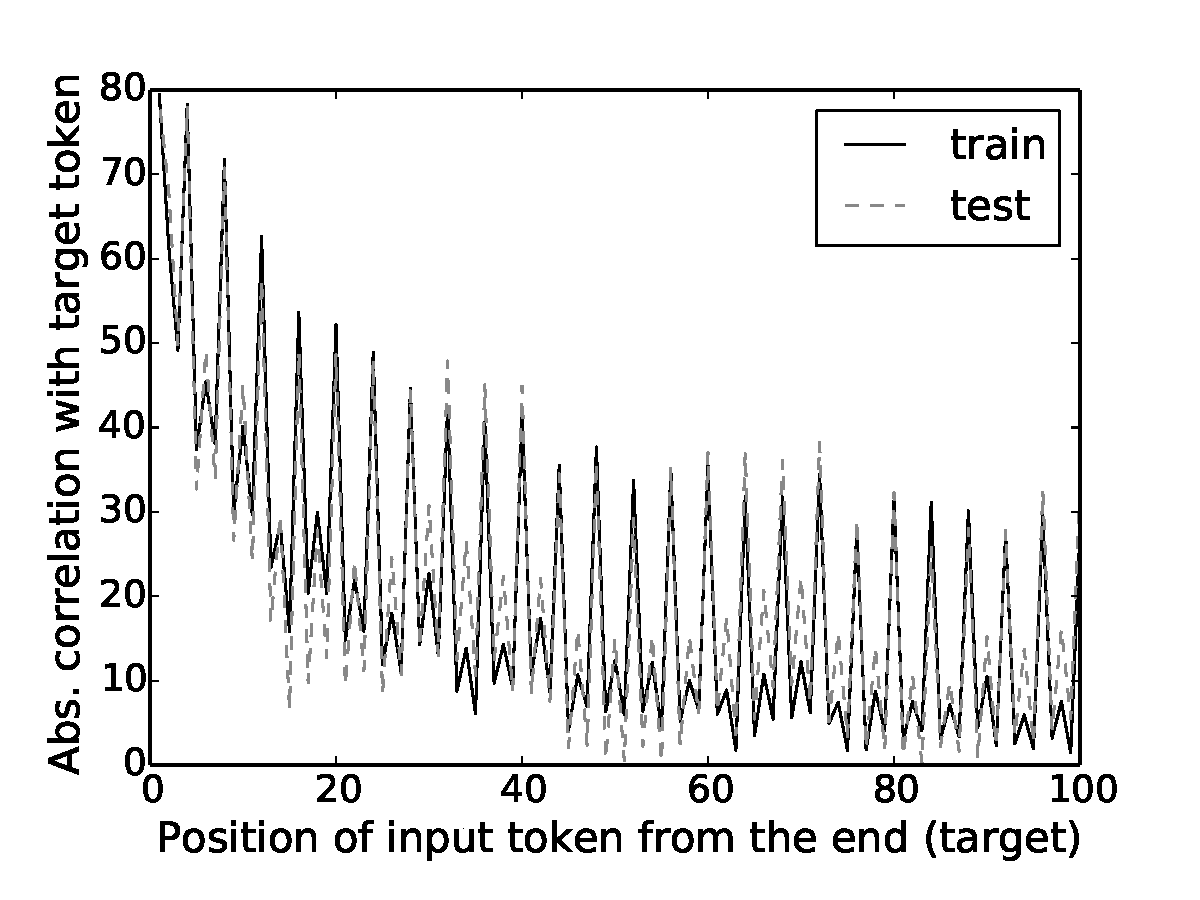
\includegraphics[width=\linewidth]{figs/correlation.pdf}
  \caption{Absolute value of correlation between input tokens and target token,
  scaled by 0.02, as a function of position of a token from the target,
  for Linux source.}
  \label{fig:correlation}
\end{figure}

\noindent
To study the influence of tokens in an incomplete piece of code on the next
(target) token, we computed the correlation between the input tokens and the
target token.
Figure~\ref{fig:correlation} shows the result (scaled absolute correlation) for
codes that we train on and codes that we test on, for Linux
source code.
We compute the correlation between every token and preceding tokens, whenever
there are at least 100 tokens before the target.
The value of a key token is between 1 and $K$, and the value of a positional
token between $K+1$ and $K+W$, with $W=100$ here.
As we expected, the absolute value of correlation between input tokens and
target token gradually decreases as the distance between them increases.
However, interestingly, when an input token is 3 tokens or more away from the
target token, tokens that are even number of tokens away (tokens 4, 6, 8, ...
from the end) have a larger magnitude of correlation with the target token.
We think this is because special characters (operators) and words such as variable and
function names typically alternate. If other projects and languages
also exhibit a similar trend, we would like to see if we can improve
predictions by considering larger windows of preceding tokens, but after
removing tokens that are odd number of tokens away from the target token.

%\vspace{-5pt}
\section{Conclusions and Future Work}
\label{sec:conclusions}

\noindent
Among the methods we tried so far, chaining two matrix-vector models with a
relu nonlinearity performs the best.
This is also the most general of all models we tried, so
the higher accuracy is not surprising. Given the results for correlation between
input and target tokens, we would like to experiment with larger windows
where we exclude odd tokens.

The word vector algorithms we tried so far do not capture file specific
patterns. Non-key tokens that are local to the file, and outside the window are
ignored. We want to try out a recurrent neural network (RNN)
approach~\cite{rnn} or a long short-term memory (LSTM) approach~\cite{lstm,
rnnlstm} to
capture file specific patterns. Another approach that we are considering is to
use file-specific word vectors --- each token in a file is a linear
transformation of its \emph{base value}, which is common across all files, and
file-specific vectors corresponding to $W$ tokens preceding it.
To predict a token, we then perform a linear transformation of file-specific
vectors corresponding to last $W$ tokens, and look for the closest
file-specific token using cosine similarity. The intuition behind this approach
is to capture local context by expressing tokens as a function of the enclosing
context. This approach resembles RNNs in some ways, and requires a forward and
a backward pass to update file-specific vectors and cost function.
File-specific vectors can be thought of as the hidden state in RNNs, but
instead of using hidden state from just the previous stage, we now use
hidden state from previous $W$ stages.

Finally, time permitting,
we would like to pick the two best algorithms, train them on different
window sizes $W$, assign a confidence to the prediction from each algorithm and
window size, and pick the prediction with the highest score.
The intuition here is that some tokens might be predicted well by
looking at a large window of preceding tokens, while some other tokens might
be predicted well by looking at a few preceding tokens (such as {\tt for}
statements).


\bibliography{milestone}
\bibliographystyle{abbrv} 

\end{document}
